% Options for packages loaded elsewhere
\PassOptionsToPackage{unicode}{hyperref}
\PassOptionsToPackage{hyphens}{url}
\PassOptionsToPackage{dvipsnames,svgnames,x11names}{xcolor}
%
\documentclass[
]{article}
\usepackage{amsmath,amssymb}
\usepackage{lmodern}
\usepackage{iftex}
\ifPDFTeX
  \usepackage[T1]{fontenc}
  \usepackage[utf8]{inputenc}
  \usepackage{textcomp} % provide euro and other symbols
\else % if luatex or xetex
  \usepackage{unicode-math}
  \defaultfontfeatures{Scale=MatchLowercase}
  \defaultfontfeatures[\rmfamily]{Ligatures=TeX,Scale=1}
\fi
% Use upquote if available, for straight quotes in verbatim environments
\IfFileExists{upquote.sty}{\usepackage{upquote}}{}
\IfFileExists{microtype.sty}{% use microtype if available
  \usepackage[]{microtype}
  \UseMicrotypeSet[protrusion]{basicmath} % disable protrusion for tt fonts
}{}
\makeatletter
\@ifundefined{KOMAClassName}{% if non-KOMA class
  \IfFileExists{parskip.sty}{%
    \usepackage{parskip}
  }{% else
    \setlength{\parindent}{0pt}
    \setlength{\parskip}{6pt plus 2pt minus 1pt}}
}{% if KOMA class
  \KOMAoptions{parskip=half}}
\makeatother
\usepackage{xcolor}
\usepackage{graphicx}
\makeatletter
\def\maxwidth{\ifdim\Gin@nat@width>\linewidth\linewidth\else\Gin@nat@width\fi}
\def\maxheight{\ifdim\Gin@nat@height>\textheight\textheight\else\Gin@nat@height\fi}
\makeatother
% Scale images if necessary, so that they will not overflow the page
% margins by default, and it is still possible to overwrite the defaults
% using explicit options in \includegraphics[width, height, ...]{}
\setkeys{Gin}{width=\maxwidth,height=\maxheight,keepaspectratio}
% Set default figure placement to htbp
\makeatletter
\def\fps@figure{htbp}
\makeatother
\setlength{\emergencystretch}{3em} % prevent overfull lines
\providecommand{\tightlist}{%
  \setlength{\itemsep}{0pt}\setlength{\parskip}{0pt}}
\setcounter{secnumdepth}{-\maxdimen} % remove section numbering
% definitions for citeproc citations
\NewDocumentCommand\citeproctext{}{}
\NewDocumentCommand\citeproc{mm}{%
  \begingroup\def\citeproctext{#2}\cite{#1}\endgroup}
\makeatletter
 % allow citations to break across lines
 \let\@cite@ofmt\@firstofone
 % avoid brackets around text for \cite:
 \def\@biblabel#1{}
 \def\@cite#1#2{{#1\if@tempswa , #2\fi}}
\makeatother
\newlength{\cslhangindent}
\setlength{\cslhangindent}{1.5em}
\newlength{\csllabelwidth}
\setlength{\csllabelwidth}{3em}
\newenvironment{CSLReferences}[2] % #1 hanging-indent, #2 entry-spacing
 {\begin{list}{}{%
  \setlength{\itemindent}{0pt}
  \setlength{\leftmargin}{0pt}
  \setlength{\parsep}{0pt}
  % turn on hanging indent if param 1 is 1
  \ifodd #1
   \setlength{\leftmargin}{\cslhangindent}
   \setlength{\itemindent}{-1\cslhangindent}
  \fi
  % set entry spacing
  \setlength{\itemsep}{#2\baselineskip}}}
 {\end{list}}
\usepackage{calc}
\newcommand{\CSLBlock}[1]{\hfill\break\parbox[t]{\linewidth}{\strut\ignorespaces#1\strut}}
\newcommand{\CSLLeftMargin}[1]{\parbox[t]{\csllabelwidth}{\strut#1\strut}}
\newcommand{\CSLRightInline}[1]{\parbox[t]{\linewidth - \csllabelwidth}{\strut#1\strut}}
\newcommand{\CSLIndent}[1]{\hspace{\cslhangindent}#1}
\ifLuaTeX
\usepackage[bidi=basic]{babel}
\else
\usepackage[bidi=default]{babel}
\fi
\babelprovide[main,import]{american}
% get rid of language-specific shorthands (see #6817):
\let\LanguageShortHands\languageshorthands
\def\languageshorthands#1{}
\ifLuaTeX
  \usepackage{selnolig}  % disable illegal ligatures
\fi
\IfFileExists{bookmark.sty}{\usepackage{bookmark}}{\usepackage{hyperref}}
\IfFileExists{xurl.sty}{\usepackage{xurl}}{} % add URL line breaks if available
\urlstyle{same} % disable monospaced font for URLs
\hypersetup{
  pdftitle={LAMMPS-GUI: A Cross-Platform Graphical Tool to Learn and
Explore Molecular Dynamics with LAMMPS},
  pdfauthor={Axel Kohlmeyer},
  pdflang={en-US},
  colorlinks=true,
  linkcolor={Maroon},
  filecolor={Maroon},
  citecolor={Blue},
  urlcolor={Blue},
  pdfcreator={LaTeX via pandoc}}

\title{LAMMPS-GUI: A Cross-Platform Graphical Tool to Learn and Explore
Molecular Dynamics with LAMMPS}

\definecolor{c53baa1}{RGB}{83,186,161}
\definecolor{c202826}{RGB}{32,40,38}
\def \rorglobalscale {0.1}
\newcommand{\rorlogo}{%
\begin{tikzpicture}[y=1cm, x=1cm, yscale=\rorglobalscale,xscale=\rorglobalscale, every node/.append style={scale=\rorglobalscale}, inner sep=0pt, outer sep=0pt]
  \begin{scope}[even odd rule,line join=round,miter limit=2.0,shift={(-0.025, 0.0216)}]
    \path[fill=c53baa1,nonzero rule,line join=round,miter limit=2.0] (1.8164, 3.012) -- (1.4954, 2.5204) -- (1.1742, 3.012) -- (1.8164, 3.012) -- cycle;
    \path[fill=c53baa1,nonzero rule,line join=round,miter limit=2.0] (3.1594, 3.012) -- (2.8385, 2.5204) -- (2.5172, 3.012) -- (3.1594, 3.012) -- cycle;
    \path[fill=c53baa1,nonzero rule,line join=round,miter limit=2.0] (1.1742, 0.0669) -- (1.4954, 0.5588) -- (1.8164, 0.0669) -- (1.1742, 0.0669) -- cycle;
    \path[fill=c53baa1,nonzero rule,line join=round,miter limit=2.0] (2.5172, 0.0669) -- (2.8385, 0.5588) -- (3.1594, 0.0669) -- (2.5172, 0.0669) -- cycle;
    \path[fill=c202826,nonzero rule,line join=round,miter limit=2.0] (3.8505, 1.4364).. controls (3.9643, 1.4576) and (4.0508, 1.5081) .. (4.1098, 1.5878).. controls (4.169, 1.6674) and (4.1984, 1.7642) .. (4.1984, 1.8777).. controls (4.1984, 1.9719) and (4.182, 2.0503) .. (4.1495, 2.1132).. controls (4.1169, 2.1762) and (4.0727, 2.2262) .. (4.0174, 2.2635).. controls (3.9621, 2.3006) and (3.8976, 2.3273) .. (3.824, 2.3432).. controls (3.7505, 2.359) and (3.6727, 2.367) .. (3.5909, 2.367) -- (2.9676, 2.367) -- (2.9676, 1.8688).. controls (2.9625, 1.8833) and (2.9572, 1.8976) .. (2.9514, 1.9119).. controls (2.9083, 2.0164) and (2.848, 2.1056) .. (2.7705, 2.1791).. controls (2.6929, 2.2527) and (2.6014, 2.3093) .. (2.495, 2.3487).. controls (2.3889, 2.3881) and (2.2728, 2.408) .. (2.1468, 2.408).. controls (2.0209, 2.408) and (1.905, 2.3881) .. (1.7986, 2.3487).. controls (1.6925, 2.3093) and (1.6007, 2.2527) .. (1.5232, 2.1791).. controls (1.4539, 2.1132) and (1.3983, 2.0346) .. (1.3565, 1.9436).. controls (1.3504, 2.009) and (1.3351, 2.0656) .. (1.3105, 2.1132).. controls (1.2779, 2.1762) and (1.2338, 2.2262) .. (1.1785, 2.2635).. controls (1.1232, 2.3006) and (1.0586, 2.3273) .. (0.985, 2.3432).. controls (0.9115, 2.359) and (0.8337, 2.367) .. (0.7519, 2.367) -- (0.1289, 2.367) -- (0.1289, 0.7562) -- (0.4837, 0.7562) -- (0.4837, 1.4002) -- (0.6588, 1.4002) -- (0.9956, 0.7562) -- (1.4211, 0.7562) -- (1.0118, 1.4364).. controls (1.1255, 1.4576) and (1.2121, 1.5081) .. (1.2711, 1.5878).. controls (1.2737, 1.5915) and (1.2761, 1.5954) .. (1.2787, 1.5991).. controls (1.2782, 1.5867) and (1.2779, 1.5743) .. (1.2779, 1.5616).. controls (1.2779, 1.4327) and (1.2996, 1.3158) .. (1.3428, 1.2113).. controls (1.3859, 1.1068) and (1.4462, 1.0176) .. (1.5237, 0.944).. controls (1.601, 0.8705) and (1.6928, 0.8139) .. (1.7992, 0.7744).. controls (1.9053, 0.735) and (2.0214, 0.7152) .. (2.1474, 0.7152).. controls (2.2733, 0.7152) and (2.3892, 0.735) .. (2.4956, 0.7744).. controls (2.6016, 0.8139) and (2.6935, 0.8705) .. (2.771, 0.944).. controls (2.8482, 1.0176) and (2.9086, 1.1068) .. (2.952, 1.2113).. controls (2.9578, 1.2253) and (2.9631, 1.2398) .. (2.9681, 1.2544) -- (2.9681, 0.7562) -- (3.3229, 0.7562) -- (3.3229, 1.4002) -- (3.4981, 1.4002) -- (3.8349, 0.7562) -- (4.2603, 0.7562) -- (3.8505, 1.4364) -- cycle(0.9628, 1.7777).. controls (0.9438, 1.7534) and (0.92, 1.7357) .. (0.8911, 1.7243).. controls (0.8623, 1.7129) and (0.83, 1.706) .. (0.7945, 1.7039).. controls (0.7588, 1.7015) and (0.7252, 1.7005) .. (0.6932, 1.7005) -- (0.4839, 1.7005) -- (0.4839, 2.0667) -- (0.716, 2.0667).. controls (0.7477, 2.0667) and (0.7805, 2.0643) .. (0.8139, 2.0598).. controls (0.8472, 2.0553) and (0.8768, 2.0466) .. (0.9025, 2.0336).. controls (0.9282, 2.0206) and (0.9496, 2.0021) .. (0.9663, 1.9778).. controls (0.9829, 1.9534) and (0.9914, 1.9209) .. (0.9914, 1.8799).. controls (0.9914, 1.8362) and (0.9819, 1.8021) .. (0.9628, 1.7777) -- cycle(2.6125, 1.3533).. controls (2.5889, 1.2904) and (2.5553, 1.2359) .. (2.5112, 1.1896).. controls (2.4672, 1.1433) and (2.4146, 1.1073) .. (2.3529, 1.0814).. controls (2.2916, 1.0554) and (2.2228, 1.0427) .. (2.1471, 1.0427).. controls (2.0712, 1.0427) and (2.0026, 1.0557) .. (1.9412, 1.0814).. controls (1.8799, 1.107) and (1.8272, 1.1433) .. (1.783, 1.1896).. controls (1.7391, 1.2359) and (1.7052, 1.2904) .. (1.6817, 1.3533).. controls (1.6581, 1.4163) and (1.6465, 1.4856) .. (1.6465, 1.5616).. controls (1.6465, 1.6359) and (1.6581, 1.705) .. (1.6817, 1.7687).. controls (1.7052, 1.8325) and (1.7388, 1.8873) .. (1.783, 1.9336).. controls (1.8269, 1.9799) and (1.8796, 2.0159) .. (1.9412, 2.0418).. controls (2.0026, 2.0675) and (2.0712, 2.0804) .. (2.1471, 2.0804).. controls (2.223, 2.0804) and (2.2916, 2.0675) .. (2.3529, 2.0418).. controls (2.4143, 2.0161) and (2.467, 1.9799) .. (2.5112, 1.9336).. controls (2.5551, 1.8873) and (2.5889, 1.8322) .. (2.6125, 1.7687).. controls (2.636, 1.705) and (2.6477, 1.6359) .. (2.6477, 1.5616).. controls (2.6477, 1.4856) and (2.636, 1.4163) .. (2.6125, 1.3533) -- cycle(3.8015, 1.7777).. controls (3.7825, 1.7534) and (3.7587, 1.7357) .. (3.7298, 1.7243).. controls (3.701, 1.7129) and (3.6687, 1.706) .. (3.6333, 1.7039).. controls (3.5975, 1.7015) and (3.5639, 1.7005) .. (3.5319, 1.7005) -- (3.3226, 1.7005) -- (3.3226, 2.0667) -- (3.5547, 2.0667).. controls (3.5864, 2.0667) and (3.6192, 2.0643) .. (3.6526, 2.0598).. controls (3.6859, 2.0553) and (3.7155, 2.0466) .. (3.7412, 2.0336).. controls (3.7669, 2.0206) and (3.7883, 2.0021) .. (3.805, 1.9778).. controls (3.8216, 1.9534) and (3.8301, 1.9209) .. (3.8301, 1.8799).. controls (3.8301, 1.8362) and (3.8206, 1.8021) .. (3.8015, 1.7777) -- cycle;
  \end{scope}
\end{tikzpicture}
}

%%%%%%%%%%%%%%%%%%%%%%%%%%%%%%%%%%%%%%%%%%%%%%%%%%%%%%%%%%%%%%%%%%%%%%%%
% Authors and Affiliations

\usepackage[affil-it]{authblk}
\usepackage{orcidlink}
%% \renewcommand\Authsep{, }
\setlength{\affilsep}{1em}
\author[1%
  %
  \ensuremath\mathparagraph]{Axel Kohlmeyer%
    \,\orcidlink{0000-0001-6204-6475}\,%
    }

\affil[1]{Institute for Computational Molecular Science, Temple
University, Philadelphia, PA, USA%
  }
\affil[$\mathparagraph$]{Corresponding author: %
   %
}
%%%%%%%%%%%%%%%%%%%%%%%%%%%%%%%%%%%%%%%%%%%%%%%%%%%%%%%%%%%%%%%%%%%%%%%%
\date{27 June 2026}

\begin{document}
\maketitle

\section{Summary}\label{summary}

LAMMPS is a widely used, massively parallel classical molecular dynamics
(MD) engine for particle-based simulations at the atomic, mesoscopic,
and continuum scales (\citeproc{ref-thompson2022lammps}{Thompson et al.,
2022}). Implemented in C++ as a no-frills, console-mode application, it
is highly portable and efficient, but learning to use it requires
mastering separate -- and often platform-specific -- tools for editing
inputs, plotting thermodynamic data, and visualizing atomic
configurations \emph{before} one can begin to learn MD itself.

LAMMPS-GUI is a cross-platform graphical application, written in C++17
using version 6 of the Qt framework (\citeproc{ref-qt_home}{The Qt
Company, 2026}), that combines these tasks in one program: a
syntax-highlighting input editor with auto-completion and documentation
lookup, live execution with real-time output monitoring, interactive
thermodynamic charts, a snapshot image viewer, and a slide-show viewer.
Rather than launching LAMMPS as an external process, it embeds the
engine through the C-language library interface
(\citeproc{ref-frantzdale2010library}{FrantzDale et al., 2010}), running
the simulation in a concurrent worker thread so the interface stays
responsive and the run can be monitored, plotted, visualized, and
cleanly stopped. By mirroring the traditional ``edit, run, observe,
analyze'' workflow, it lets users move freely to the command-line
executable -- essential once a workflow outgrows a personal computer.
Pre-compiled packages for Windows, macOS, and Linux let most users start
instantly, without compiling anything.

\section{Statement of need}\label{statement-of-need}

LAMMPS-GUI grew out of teaching LAMMPS at tutorials and workshops, where
much of the available time went not to molecular dynamics but to
installing and operating the surrounding tool chain -- a text editor, a
plotting program, and a molecular visualization package -- most of which
differ between Windows, macOS, and Linux. Earlier workarounds were
either too complex to sustain or broke when Apple moved to the ARM
architecture. As a single, self-contained, cross-platform tool that
mirrors the console workflow, LAMMPS-GUI removes this barrier, letting
instructors teach one interface on all platforms and focus on LAMMPS and
molecular dynamics itself.

\begin{figure}
\centering
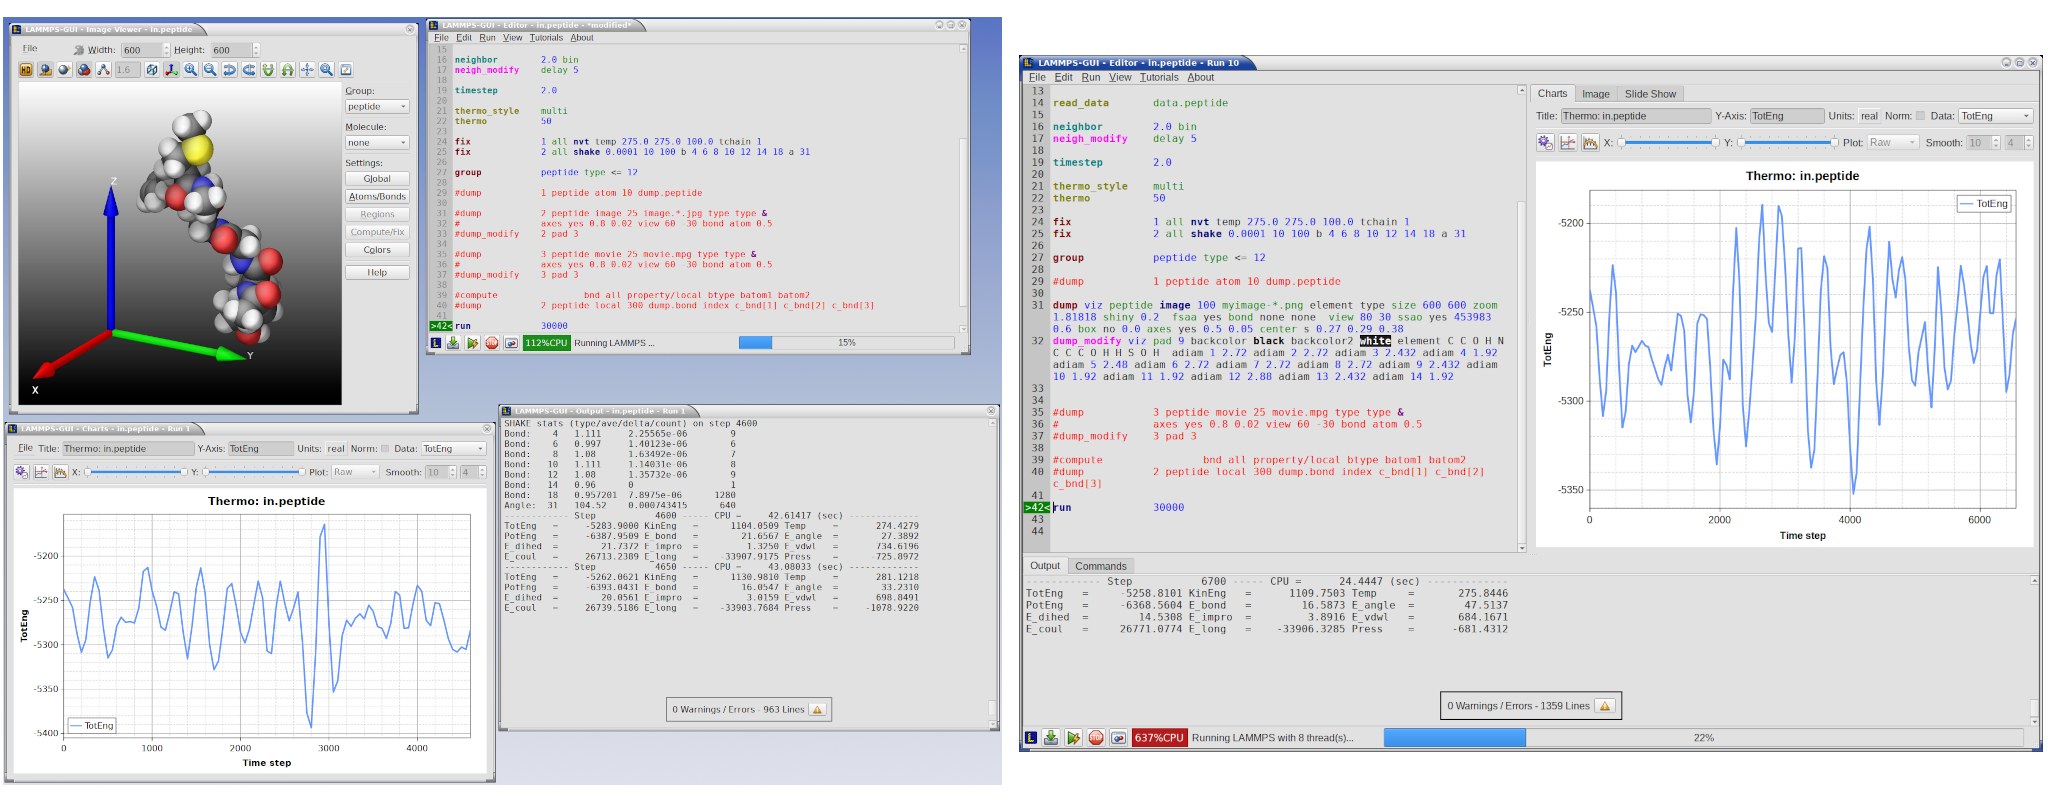
\includegraphics[width=0.99\linewidth,height=\textheight,keepaspectratio]{images/lammps-gui-screen.png}
\caption{A LAMMPS-GUI session with a simulation in flight, in the
individual window mode (left) and the combined window mode (right). The
editor shows syntax highlighting, line numbers, and a marker on the
current input line; the status bar shows CPU utilization and run
progress; the Image Viewer shows the starting geometry, the Output
window the screen output, and the Charts window a live plot of a
thermodynamic column. In the combined window mode these views are tabs
beside and below the editor.\label{fig:editor}}
\end{figure}

\section{State of the field}\label{state-of-the-field}

Other approaches to making LAMMPS more accessible exist, but they target
different needs. Commercial molecular-modeling packages provide
structure editors that export LAMMPS inputs and re-import results;
Atomify compiles a modified LAMMPS to WebAssembly and runs simulations
and visualization inside a web browser
(\citeproc{ref-atomify_home}{Hafreager, 2025}); and dedicated
visualization programs such as OVITO
(\citeproc{ref-ovito2010}{Stukowski, 2010}) and VMD
(\citeproc{ref-vmd1996}{Humphrey et al., 1996}) render trajectories with
a breadth and quality that LAMMPS-GUI does not attempt to match. None of
these, however, integrates input editing, live simulation, output
monitoring, plotting, and visualization into one application that
follows the same edit-run-observe loop as the standalone executable.
LAMMPS-GUI fills that gap. It also imports tutorial materials, such as
the official LAMMPS tutorials
(\citeproc{ref-gravelle2025lammps}{Gravelle et al., 2025}) on molecular
soft matter, with collections on materials science and discrete element
modeling in preparation. Although aimed primarily at beginners, features
such as rapid prototyping of input decks, debugging failing inputs by
visualizing selected components, and interactive construction of
reproducible \texttt{dump\ image} commands also make it useful to
experienced researchers.

\section{Software design and
functionality}\label{software-design-and-functionality}

LAMMPS-GUI follows an object-oriented design in which a central window
coordinates largely self-contained components, all access to LAMMPS
being funneled through a single adapter class. Two viewing modes are
offered: the original individual window mode, where every component is a
window of its own, and a recently added combined window mode, where the
views are docked as tabbed panels beside and below the editor in one
main window, separated by movable splitters. Key capabilities of
LAMMPS-GUI include:

\begin{itemize}
\tightlist
\item
  \textbf{Editing.} A LAMMPS-aware editor with syntax highlighting,
  per-command-category auto-completion, in-place documentation lookup,
  block comment/uncomment, and command reformatting.
\item
  \textbf{Running.} Execution of the editor buffer through the library
  interface with no intermediate file I/O, a progress bar with estimated
  completion, support for the GPU, INTEL, KOKKOS, and OPENMP accelerator
  packages, and recovery from simulation errors -- reported as catchable
  exceptions -- without crashing.
\item
  \textbf{Output and charts.} An output window that highlights warnings
  and errors and makes documentation URLs clickable, and a charts window
  that plots thermodynamic data read directly from the running
  simulation (not scraped from text) or from external files, with
  Savitzky-Golay smoothing (\citeproc{ref-savitzkygolay1964}{Savitzky \&
  Golay, 1964}) and post-processing such as autocorrelation functions,
  Fourier transforms, static structure factors, and polynomial,
  Birch-Murnaghan equation-of-state, and custom nonlinear fits.
\item
  \textbf{Visualization.} A snapshot image viewer that builds
  high-quality renderings via the LAMMPS \texttt{dump\ image} command,
  with interactive controls and the ability to copy the generated
  command back into the script for reproducible figures, plus a
  slide-show viewer that plays image sequences, imports frames from
  movie files, and exports movies.
\item
  \textbf{Tutorials and convenience.} A guided wizard that downloads
  lesson inputs from several tutorial collections, a tabbed preferences
  dialog, hand-off of the current system to OVITO and VMD, and
  command-line flags exposing the charting, slide-show, and text viewers
  as standalone utilities.
\end{itemize}

What LAMMPS-GUI deliberately does not provide is a molecular editor or
builder. Creating complex, physically sound initial configurations with
their topology has never been within the scope of LAMMPS, and the GUI
does not address it either. The built-in lattice, region, and molecule
template commands cover many cases; beyond those, and especially for the
atom typing and partial charge assignment that molecular force fields
require, force-field specific external tools are needed, for which the
LAMMPS website maintains a curated list
(\citeproc{ref-lammps_home_prepost}{LAMMPS Developers, 2026a}).

A recurring theme is the co-evolution of LAMMPS-GUI and LAMMPS:
front-end needs drove improvements to the engine and its library
interface -- catchable exceptions, a locked cache of live thermodynamic
data, and greatly expanded snapshot rendering, collected into a
dedicated GRAPHICS package (\citeproc{ref-kohlmeyer2025lammps}{Kohlmeyer
\& Berger, 2025}), which brings functionality long provided by dedicated
visualization tools directly to a running simulation rather than only to
saved trajectory files. In its default \emph{plugin mode}, LAMMPS-GUI
loads the shared library at run time with no link-time dependency, so
one binary can pair with -- or download -- different LAMMPS builds.

\section{Research impact statement}\label{research-impact-statement}

LAMMPS-GUI has shipped with LAMMPS since the August 2023 stable release,
first from within the LAMMPS source tree and since August 2025 as an
independently versioned package that the LAMMPS build system fetches on
request; the pre-compiled LAMMPS packages for Windows, macOS, and Linux
posted with each LAMMPS release bundle it
(\citeproc{ref-lammps_releases}{LAMMPS Developers, 2026b}). It is the
primary tool of the peer-reviewed LAMMPS tutorials
(\citeproc{ref-gravelle2025lammps}{Gravelle et al., 2025}), which are
written around it, and it has anchored public hands-on training since
the 2024 LAMMPS master class, including the tutorial session of the 2025
LAMMPS Workshop and Symposium (\citeproc{ref-lammps_workshop2025}{LAMMPS
Developers, 2025}); recordings of both live streams are online
(\citeproc{ref-templelammps_streams}{Temple LAMMPS, 2024}). Its
development has also fed improvements back into the LAMMPS engine
itself, as described above. The project is maintained as research
software: a documentation site (\citeproc{ref-lammpsgui_home}{Kohlmeyer,
2026}), releases archived on Zenodo, continuous-integration builds and
automated tests on all three platforms, and user support through a
dedicated tag on the LAMMPS forum.

\section{AI usage disclosure}\label{ai-usage-disclosure}

The design and architecture of LAMMPS-GUI were developed without the use
of generative AI. However, AI-based coding assistants such as GitHub
Copilot and Claude Code were used more recently to support the
refactoring and modularization of the existing code base, and to assist
with editing this manuscript. All AI-generated suggestions were
reviewed, tested, and revised by the author, who takes full
responsibility for the software and for the content of this paper.

\section{Acknowledgements}\label{acknowledgements}

Financial support by Sandia National Laboratories under PO 2149742 and
PO 2407526, by the US National Science Foundation via Major Research
Infrastructure grants number 1625061 and 2216289, and by CCDC-ARL under
Cooperative Agreement Number W911NF-21-2-0007 is gratefully
acknowledged. The author thanks the LAMMPS developers and the authors of
the LAMMPS tutorials for their feedback and for motivating many of the
features described here.

\section*{References}\label{references}
\addcontentsline{toc}{section}{References}

\protect\phantomsection\label{refs}
\begin{CSLReferences}{1}{0}
\bibitem[\citeproctext]{ref-frantzdale2010library}
FrantzDale, B., Plimpton, S. J., \& Shephard, M. S. (2010). Software
components for parallel multiscale simulation: An example with {LAMMPS}.
\emph{Engineering with Computers}, \emph{26}, 205--211.
\url{https://doi.org/10.1007/s00366-009-0156-z}

\bibitem[\citeproctext]{ref-gravelle2025lammps}
Gravelle, S., Alvares, C. M. S., Gissinger, J. R., \& Kohlmeyer, A.
(2025). A set of tutorials for the {LAMMPS} simulation package.
\emph{Living Journal of Computational Molecular Science}, \emph{6}(1),
3037. \url{https://doi.org/10.33011/livecoms.6.1.3037}

\bibitem[\citeproctext]{ref-atomify_home}
Hafreager, A. (2025). \emph{Atomify}.
\url{https://andeplane.github.io/atomify}

\bibitem[\citeproctext]{ref-vmd1996}
Humphrey, W., Dalke, A., \& Schulten, K. (1996). {VMD}: Visual molecular
dynamics. \emph{Journal of Molecular Graphics}, \emph{14}(1), 33--38.
\url{https://doi.org/10.1016/0263-7855(96)00018-5}

\bibitem[\citeproctext]{ref-lammpsgui_home}
Kohlmeyer, A. (2026). \emph{{LAMMPS-GUI} documentation}.
\url{https://lammps-gui.lammps.org/}

\bibitem[\citeproctext]{ref-kohlmeyer2025lammps}
Kohlmeyer, A., \& Berger, R. (2025). {LAMMPS}: A case study for applying
modern software engineering to an established research software package.
\emph{US Research Software Engineering Conference (US-RSE'25),
Philadelphia, PA, USA}. \url{https://doi.org/10.5281/zenodo.17410115}

\bibitem[\citeproctext]{ref-lammps_workshop2025}
LAMMPS Developers, T. (2025). \emph{{LAMMPS} workshop and symposium,
august 12-14, 2025: Tutorial session}.
\url{https://www.lammps.org/workshops/Aug25/tutorial/}

\bibitem[\citeproctext]{ref-lammps_home_prepost}
LAMMPS Developers, T. (2026a). \emph{{LAMMPS} homepage - pre- and
post-processing tools}. \url{https://www.lammps.org/ecosystem/prepost/}

\bibitem[\citeproctext]{ref-lammps_releases}
LAMMPS Developers, T. (2026b). \emph{{LAMMPS} releases on {GitHub}}.
\url{https://github.com/lammps/lammps/releases}

\bibitem[\citeproctext]{ref-savitzkygolay1964}
Savitzky, A., \& Golay, M. J. E. (1964). Smoothing and differentiation
of data by simplified least squares procedures. \emph{Analytical
Chemistry}, \emph{36}(8), 1627--1639.
\url{https://doi.org/10.1021/ac60214a047}

\bibitem[\citeproctext]{ref-ovito2010}
Stukowski, A. (2010). Visualization and analysis of atomistic simulation
data with {OVITO} -- the open visualization tool. \emph{Modelling and
Simulation in Materials Science and Engineering}, \emph{18}(1), 015012.
\url{https://doi.org/10.1088/0965-0393/18/1/015012}

\bibitem[\citeproctext]{ref-templelammps_streams}
Temple LAMMPS. (2024). \emph{{LAMMPS} tutorial live streams}. YouTube.
\url{https://www.youtube.com/@templelammps/streams}

\bibitem[\citeproctext]{ref-qt_home}
The Qt Company. (2026). \emph{Qt cross-platform framework}.
\url{https://www.qt.io/}

\bibitem[\citeproctext]{ref-thompson2022lammps}
Thompson, A. P., Aktulga, H. M., Berger, R., Bolintineanu, D. S., Brown,
W. M., Crozier, P. S., Veld, P. J. in't, Kohlmeyer, A., Moore, S. G.,
Nguyen, T. D., Shan, R., Stevens, M. J., Tranchida, J., Trott, C., \&
Plimpton, S. J. (2022). {LAMMPS} -- a flexible simulation tool for
particle-based materials modeling at the atomic, meso, and continuum
scales. \emph{Computer Physics Communications}, \emph{271}, 108171.
\url{https://doi.org/10.1016/j.cpc.2021.108171}

\end{CSLReferences}

\end{document}
